\chapter{Beschreibung der verschiedenen Messungen und Ergebnisdarstellung}

\section{Konfiguration der Router}
Die folgenden Schritte sind bei allen Routern durchzuf�hren. Gezeigt wird
beispielhaft die Vorgehensweise f�r Router 1.
\subsection{Basiskonfiguration}
Zun�chst ist der Hostname zu R1 zu �ndern. Anschlie�end werden die Passw�rter
konfiguriert und ``logging synchronous'' aktiviert.
\begin{lstlisting}
Router>enable
Router#configure terminal
Router(config)# hostname R1
R1(config)#line console 0
R1(config-line)#password cisco
R1(config-line)#login
R1(config-line)#exit
R1(config)#line vty 0 4
R1(config-line)#password cisco
R1(config-line)#login
R1(config)#enable password cisco
R1(config)#enable secret class
R1(config)#exit
R1(config)#line console 0
R1(config-line)#logging synchronous
\end{lstlisting}
F�r die Konsole wird das Passwort ``cisco'', f�r den Priviledged EXEC Mode
``class'', vergeben. Durch ``logging synchronous'' wird sichergestellt, dass
keine Systemnachrichten die Befehlseingabe unterbrechen.
\newline
Um die Weiterleitung von IPv6-Paketen zu erm�glichen, muss im \acs{CLI} des
Routers das Kommando \textit{ipv6 unicast-routing} ausgef�hrt werden.
\newline
Router 2 und Router 3 werden �uivalent konfiguriert.

\subsection{Fast-Ethernet-Schnittstelle}\label{FE}
Im Configuration Mode wird die Fast-Ethernet-Schnittstelle 0/0 konfiguriert
und die entsprechende IPv6-Adresse, sowie die Link-Local-Adresse, aus \ref{config1}
zugewiesen:
\begin{lstlisting}
R1(config)#interface FastEthernet 0/0
R1(config-if)#description R1 LAN Default Gateway
R1(config-if)#R1(config-if)# ipv6 address 2001:DB8:1:1::1/64
R1(config-if)# ipv6 address FE80::1 link-local
R1(config-if)#no shutdown
R1(config-if)#exit
R1(config)#exit
\end{lstlisting}
\subsection{Serial-Schnittstelle}
Analog zu \ref{FE} wird die Serial-Schnittstelle 0/0/0 konfiguriert:
\begin{lstlisting}
R1(config)#interface serial 0/0/0
R1(config-if)#description WAN link to R2
R1(config-if)#ipv6 address 2001:DB8:1:A001::1/64
R1(config-if)#clock rate 64000
R1(config-if)#no shutdown
R1(config-if)#exit
R1(config)#exit
\end{lstlisting}

\section{Konfiguration der Hosts}
Den Hosts wird das jeweilige Default Gateway (Link-Local-Adresse des Routers)
und die entsprechende statische IPv6-Adresse gem�� \ref{config1} zugewiesen. 

\section{Netzwerk-Konfiguration �berpr�fen}

\subsection{�berpr�fung mittels Ping-Befehlen}
Zun�chst wird mittels Eingabeaufforderung �berpr�ft, ob die Konfiguration der
Hosts korrekt ist.\footnote{siehe Anhang \ref{ipconfig}}
\newline
Danach werden Ping-Befehle ausgef�hrt um die Konfiguration zu testen:
\begin{itemize}
  \item PC1 zu R1
  \item PC2 zu R2
  \item PC3 zu R3
\end{itemize}
Die Befehle verlaufen alle erfolgreich.\footnote{siehe Anhang \ref{pingrouter}}
\clearpage
\section{Schnittstellen-Konfiguration �berpr�fen}\label{multi}
Durch \textit{show ipv6 interface brief} l�sst sich der Status der Interfaces
�berpr�fen:
\begin{lstlisting}
R1#sh ipv6 interface brief
FastEthernet0/0            [up/up]
    FE80::1
    2001:DB8:1:1::1
FastEthernet0/1            [administratively down/down]
Serial0/0/0                [up/up]
    FE80::290:2BFF:FE95:C001
    2001:DB8:1:A001::1
Serial0/0/1                [administratively down/down]
Vlan1                      [administratively down/down]
\end{lstlisting}

Bei der Fast-Ethernet-Schnittstelle 0/0 werden zwei IPv6-Adressen angezeigt, die
Link-Local-Adresse und die zuvor konfigurierte IP-Adresse der Schnittstelle.
\newline
\newline
Durch \textit{show ipv6 interface} erh�lt man mehr Informationen zu der
Schnittstellen-Konfiguration. Der folgende Auszug bezieht sich auf die
Fast-Ethernet-Schnittstelle 0/0:
\begin{lstlisting}
R1#sh ipv6 interface 
FastEthernet0/0 is up, line protocol is up
  IPv6 is enabled, link-local address is FE80::1
  No Virtual link-local address(es):
  Global unicast address(es):
    2001:DB8:1:1::1, subnet is 2001:DB8:1:1::/64
  Joined group address(es):
    FF02::1
    FF02::2
    FF02::1:FF00:1
  MTU is 1500 bytes
  ICMP error messages limited to one every 100 milliseconds
  ICMP redirects are enabled
  ICMP unreachables are sent
  ND DAD is enabled, number of DAD attempts: 1
  ND reachable time is 30000 milliseconds
  ND advertised reachable time is 0 milliseconds
  ND advertised retransmit interval is 0 milliseconds
  ND router advertisements are sent every 200 seconds
  ND router advertisements live for 1800 seconds
  ND advertised default router preference is Medium
  Hosts use stateless autoconfig for addresses.
[...]
\end{lstlisting}
Bei Router 1 werden drei Multicast-Adressen bei der
Fast-Ethernet-Schnittstelle 0/0 angezeigt:
\begin{itemize}
  \item FF02::1
  \item FF02::2
  \item FF02::1:FF00:1
\end{itemize}

\clearpage
Um die Multicast-Adressen zu identifizieren, wird das allgemeine Format einer
IPv6-Multicast-Adresse betrachtet:\cite[12]{RFC4291}

\begin{figure}[!htbp]
  \centering
     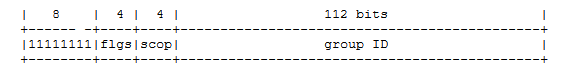
\includegraphics[width=\linewidth]{Graphics/multicast_frame.PNG}
  \caption{Format einer IPv6 Mulicast-Adresse}
  \label{fig:multicast}
\end{figure}

Eine Multicast-Adresse beginnt immer mit FF. Daruf folgt ein 4 Bit langes Flag.
Die ersten zwei Bit des Flags m�ssen 0 sein.
Der Scope ist bei allen aufgef�hrten Adressen 2, d.h. es handelt sich um einen
Link-Local Multicast-Scope.\cite[13]{RFC4291}
\newline
FF02::1 ist eine ``All-Nodes'' Multicast-Adresse.\cite[15]{RFC4291}
Diese Adresse ist vergleichbar mit der Broadcast-Adresse bei IPv4.
\newline
FE02::2 bezeichnet man als ``All-Routers'' Multicast-Adresse.\cite[15]{RFC4291}
\newline
Die dritte aufgef�hrte Multicast-Adresse FF02::1:FF00:1 ist eine
``Solicited-Node' Multicast-Adresse.\cite[15]{RFC4291}

\subsection{Solicited-Node-Adressen}\label{solicited}
In der Versuchsanleitung sind zwei weitere Multicast-Adressen
gegeben:\footnote{siehe Versuchsanleitung S.14}
\begin{itemize}
  \item FF02::1:FF00:1
  \item FF02::1:FF0D:1A60
\end{itemize}
Es handelt sich um sog. ``Solicited-Node''-Adressen.\parencite[15]{RFC4291}
\newline
Solicited-Node-Adresse sind Multicast-Adressen, die aus Unicast- und
Anycast-Adresse des PCs gebildet werden. Die niederwertigsten 24 Bit der
Unicast-oder Anycast-Adresse werden dem 104 Bit langen Pr�fix
(FF02:0:0:0:0:1:FF00::/104) angeh�ngt. Dadurch ergibt sich folgender
Wertebereich:\cite{RFC4291}\cite{RFC2461}
\newline
FF02:0:0:0:0:1:FF00:0000 bis
FF02:0:0:0:0:1:FFFF:FFFF
\newline
Solicited-Node-Adressen werden beim \ac{NDP} verwendet.\cite{RFC2461}
\newline
Das \acs{NDP} ist vergleichbar mit dem \ac{ARP} bei IPv4. Es dient unter anderem
der Adressaufl�sung.
\clearpage
\section{Konfiguration von IPv6-Routing}

\subsection{Statische Routen}
Zun�chst wird eine statische Route von Router 1 zum Netzwerk von Router 2
konfiguriert, ausgehend von der Serial-Schnittstelle 0/0/0.

\begin{lstlisting}
R1(config)#ipv6 route 2001:DB8:1:2::1/64 Serial 0/0/0
\end{lstlisting}

Anschlie�end existiert ein entsprechender Eintrag in der Routingtabelle von
Router 1:

\begin{lstlisting}
R1#sh ipv6 route
[...]
S   2001:DB8:1:2::/64 [1/0]
     via ::, Serial0/0/0
[...]
\end{lstlisting}

Danach wird ein Ping von R1 zu R2 gesendet. Dieser Versuch scheitert, da noch
keine Route von R2 zu R1 bekannt ist.
\newline
\newline
Aus diesem Grund wird im Anschluss eine statsche Route von R2 zu R1
konfiguriert:
\begin{lstlisting}
R2(config)#ipv6 route 2001:DB8:1:1::1/64 serial 0/0/0
\end{lstlisting}

Im Anschluss werden die fehlenden statischen Routen eingerichtet,
um sicherzustellen, dass alle Ger�te im Netzwerk erreichbar sind:
\begin{itemize}
  \item R1 zu R3
  \begin{lstlisting}
  R1(config)#ipv6 route 2001:DB8:1:3::1/64 serial 0/0/0
  \end{lstlisting}
  \item R3 zu R1
  \begin{lstlisting}
  R3(config)#ipv6 route 2001:DB8:1:1::1/64 serial 0/0/0
  \end{lstlisting}
    \item R2 zu R3
  \begin{lstlisting}
  R2(config)#ipv6 route 2001:DB8:1:3::1/64 serial 0/0/1
  \end{lstlisting}
  \item R3 zu R2
   \begin{lstlisting}
  R3(config)#ipv6 route 2001:DB8:1:2::1/64 serial 0/0/0
  \end{lstlisting}
\end{itemize}
\subsubsection{Konfiguration �berpr�fen}
Mittels Ping-Befehlen wird �berpr�ft, ob die Konfiguration der statischen Routen
erfolgreich war und die Ger�te erreichbar sind:
\begin{itemize}
  \item PC1 zu PC3
  \item PC3 zu PC2
\end{itemize}
Beide Versuche sind erfolgreich.\footnote{siehe Anhang \ref{pingstatic}}
\clearpage
\subsection{Default Routen}
Alle statischen Routen werden aus der Routingtabelle von R1 entfernt:
\begin{lstlisting}
R1(config)#no ipv6 route 2001:DB8:1:2::1/64 Serial 0/0/0
R1(config)#no ipv6 route 2001:DB8:1:3::1/64 serial 0/0/0
\end{lstlisting}
Danach wird eine Default-Route angelegt:
\begin{lstlisting}
R1(config)#ipv6 route ::/0 Serial 0/0/0
\end{lstlisting}

Die Routingtabelle von Router 1 enth�lt anschlie�end die neu konfigurierte
Route:
\begin{lstlisting}
R1#show ipv6 route
[...]
S   ::/0 [1/0]
     via ::, Serial0/0/0
[...]
\end{lstlisting}

Auch die konfigurierte Deafult-Route ist eine statische Route (gekennzeichnet
mit S). Das ausgehende Interface bei Host 1 ist die Serial-Schnittstelle 0/0/0.
\newline
Wenn keine definierte Route f�r ein Paket existiert, wird das Paket �ber das
Interface der Default-Route (hier S0/0/0) versandt.

\subsubsection{Konfiguration �berpr�fen}
Auch die Default Route wird mittels Ping-Befehl �berpr�ft:
\begin{itemize}
  \item PC1 zu PC2
  \item PC2 zu PC1
  \item PC1 zu PC3
  \item PC3 zu PC1
\end{itemize}
Alle Versuche sind erfolgreich.\footnote{siehe Anhang \ref{pingdefault}}